% Texcount to include the tables
%TC:group table 0 1
%TC:group longtable 0 1

\chapter{Testing and Evaluation}
\label{ch:testing-and-evaluation}
To test and evaluate the effectiveness of the proposed solution and implementation, both functional unit tests and
agent training evaluation have been used. To confirm that the environment, agents and training all work as intended,
Unit testing has been implemented in Section~\ref{sec:functional-testing}.\\
Section~\ref{sec:agent-evaluation} compares both Flexible and Fixed resource allocation problems in
Subsection~\ref{subsec:fixed-vs-flexible-resource-allocation-optimisation-problems} and agents with
different training hyperparameters (subsection~\ref{subsec:environment-and-agent-number-training}), Reinforcement
Learning algorithms (subsection~\ref{subsec:training-reinforcement-learning-algorithms}) and Neural Network
Architectures (subsection~\ref{subsec:neural-network-architecture-training}).

\section{Functional Testing}
\label{sec:functional-testing}
To confirm that the implementation of the agents and environment correctly, PyTest, a Python module, has been used. These
tests are split into three families: agent, environment and training that are
explained in their respective Tables~\ref{tab:agent-unit-tests},~\ref{tab:environment-unit-tests}
and~\ref{tab:training-unit-tests}.

\begin{longtable}{|p{3cm}|p{11cm}|} \hline
    \textbf{Unit Test name} & \textbf{Description} \\ \hline
    Building agents & Constructs all of the agents with any arguments to confirm agents can accept of all its
        attributes due to multi-inheritance means that only certain arguments are valid for each superclass. \\ \hline
    Saving agents & Confirms that agents can successfully save their neural networks and load
        the network again. \\ \hline
    Agent actions & Confirms that all agents can generate valid actions for both bidding and weighting of tasks for
        both training and evaluation. \\ \hline
    Gin config file & Gin is used to set agent and function arguments during training. To test that the
        file can be successfully parsed and arguments set. \\ \hline
    Building networks & Constructs all of the neural networks to confirm that the network accept and return valid
        inputs and outputs. \\ \hline
    Agent epsilon policy & While training agents randomly select actions in order to explore the state space.
        To tests that the random actions selected are valid and that the exploration factor (epsilon) reduces at a
        linear rate over time correctly. \\ \hline
    \caption{Table of Unit tests for Auction and Resource Allocation Agents}
    \label{tab:agent-unit-tests}
\end{longtable}

\begin{longtable}{|p{3cm}|p{11cm}|} \hline
    \textbf{Unit Test name} & \textbf{Description} \\ \hline
    Saving and loading of environments & The online flexible resource allocation environment can be saved to a
        file in its current state: server allocations, future task auctions, time steps and total time steps. This
        tests that the environment can save and loaded again. \\ \hline
    Loading environment settings & Tests that environment settings can be loaded correctly generating a new random
        environment. \\ \hline
    Random action environment steps & Tests that inputs to the auction and resource allocation steps work,
        random actions are generated to check for unknown edge cases.  \\ \hline
    Auction step & To confirm the Vickrey auction mechanism is correctly implemented, a range of edges cases
        are tested to confirm that right price is set and the task is allocated to the correct server in all cases.
        \\ \hline
    Resource allocation step & To confirm the resource allocation step is correct generate the updated state and reward
        tasks in all cases.
        \\ \hline
    Allocation of computational resources & Checks that the servers correctly allocates computational resources to
        allocated tasks given resource weightings. \\ \hline
    Allocation of storage and bandwidth resources & Checks that the servers correctly allocates storage and
        bandwidth resources to allocated tasks given resource weightings. \\ \hline
    Allocation of all resources & Checks that resources are allocated by the servers correctly given a weighting
        input for storage, computation and bandwidth resources. \\ \hline
    \caption{Table of Unit tests for the Online Flexible Resource Allocation Environment}
    \label{tab:environment-unit-tests}
\end{longtable}

\begin{longtable}{|p{3cm}|p{11cm}|} \hline
    \textbf{Unit Test name} & \textbf{Description} \\ \hline
    Task pricing training & Tests that the task pricing reinforcement learning agents correctly learning and train
        with different auction observations. \\ \hline
    Resource allocation training & Tests that resource allocation reinforcement learning agents correctly learn and
        train with different resource allocation observations. \\ \hline
    Agent evaluation & Tests that the agent evaluation function during training correctly captures information from the
        actions taken. \\ \hline
    Agent training & Tests that agents correctly train over an environment with different actions and observations.
        \\ \hline
    Random actions training & Tests random action agents using the environment training function to confirm
        that the function work as intended. \\ \hline
    \caption{Table of Unit tests for Agent training}
    \label{tab:training-unit-tests}
\end{longtable}

\section{Agent evaluation}
\label{sec:agent-evaluation}
Subsection~\ref{subsec:fixed-vs-flexible-resource-allocation-optimisation-problems},
compares the proposed Online Flexible Resource Allocation environment to an Online Fixed Resource Allocation
environment using a linear programming solver to evaluate the effectiveness of the proposed optimisation problem. \\
In order to compare the implemented agents from
Chapter~\ref{ch:implementing-flexible-resource-allocation-environment-and-server-agents}, a range of performance metrics
are recorded each time the agents are evaluated during training. These metrics are: number of failed tasks, number
of completed tasks, percentage of tasks attempted and a histogram of actions taken which together are used to compare
the performance between different agents. Differences in Server agents are compared over training environment settings
and number of agents, Reinforcement Learning algorithms and network architectures within
Subsections~\ref{subsec:environment-and-agent-number-training}
,~\ref{subsec:training-reinforcement-learning-algorithms} and~\ref{subsec:neural-network-architecture-training}
respectively.

\subsection{Fixed Vs Flexible Resource Allocation Optimisation Problems}
\label{subsec:fixed-vs-flexible-resource-allocation-optimisation-problems}
Due to tasks containing only the required resources for their lifetime instead of the proposed resource usage as in a
fixed resource allocation scheme. It is difficult to convert the Flexible Resource Allocation Optimisation problem from
Section~\ref{sec:resource-allocation-optimisation-problem}.
\hyperref[app:fixed-resource-allocation-optimisation-problem]{Appendix D} describes the conversation process for tasks
and the Fixed Resource Allocation Optimisation problem with solutions found using an integer programming solver. However
due to the complexity a time limit of 2.5 minutes were used meaning that all solution are not optimal. For the flexible
environment, a Dqn agent for both auctions and resource allocation were used.

\begin{figure}[H]
    \centering
    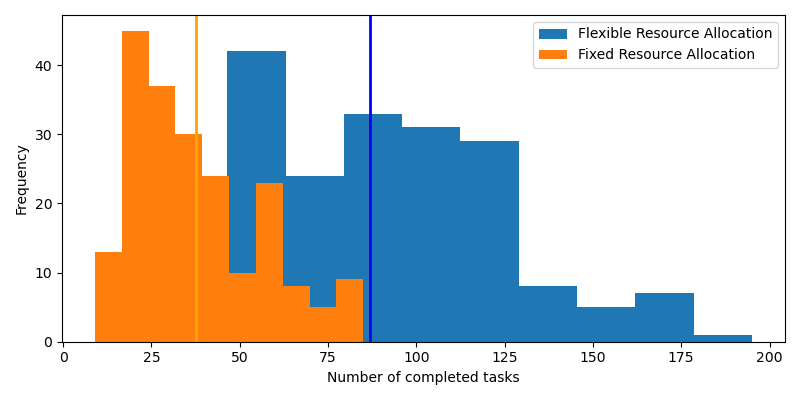
\includegraphics[width=\textwidth]{figures/5_evaluation_figs/fixed_flexible_completed_tasks.png}
    \caption{Number of Tasks completed with Fixed and Flexible resource allocation}
    \label{fig:number-task-completed-fixed-flexible}
\end{figure}

\begin{figure}[H]
    \centering
    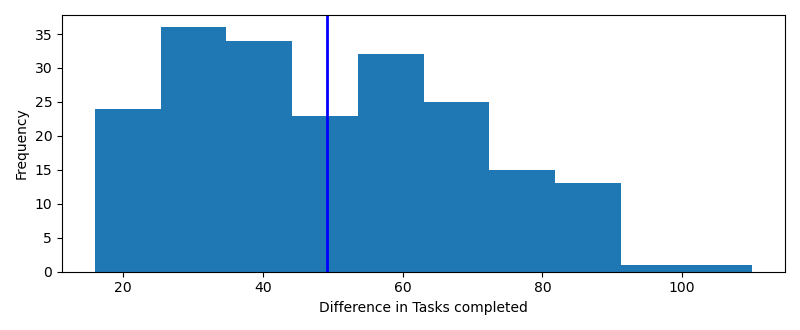
\includegraphics[width=\textwidth]{figures/5_evaluation_figs/fixed_flexible_tasks_difference.png}
    \caption{Difference in number of tasks completed in environment by the Fixed and the Flexible resource allocation agents}
    \label{fig:difference-number-task-completed-fixed-flexible}
\end{figure}

\begin{figure}[H]
    \centering
    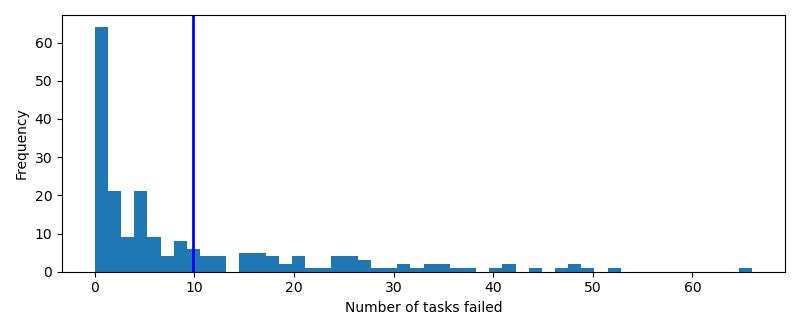
\includegraphics[width=\textwidth]{figures/5_evaluation_figs/flexible_failed_tasks.png}
    \caption{Number of tasks failed by the Flexible resource allocation agents}
    \label{fig:flexibe-failed-tasks}
\end{figure}

\begin{figure}[H]
    \centering
    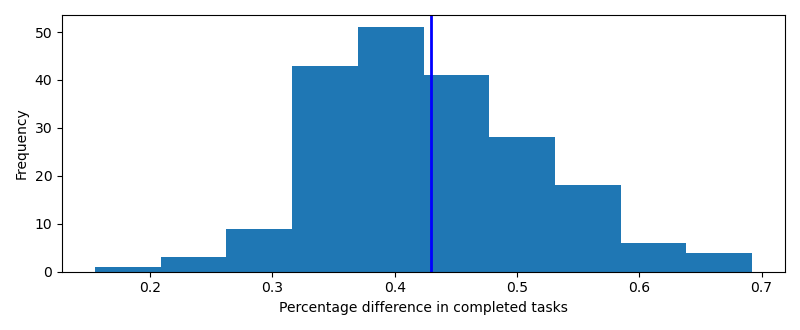
\includegraphics[width=\textwidth]{figures/5_evaluation_figs/percent_difference.png}
    \caption{Percentage difference between the number of Completed tasks by the Fixed and Flexible resource allocation}
    \label{fig:completed-percent-difference}
\end{figure}

A histogram of the number of tasks completed by the Fixed and Flexible resource allocation in
Figure~\ref{fig:number-task-completed-fixed-flexible} shows that using flexible resource allocation on average
over twice the number of tasks can be completed per environment, 35 to 81.
Figure~\ref{fig:difference-number-task-completed-fixed-flexible} shows the difference in the number of tasks completed
per environment, with on average 51 more tasks being completed by the flexible resource allocation. However on average
the flexible resource allocation also fails 10 tasks per environment, as shown in Figure~\ref{fig:flexibe-failed-tasks}
with in some cases significantly more. \\
While these results show that the Flexible resource allocation has significantly better results than the Fixed resource
allocation. The results need further analyse to confirm as the fixed resource allocation is not a perfect conversation
from the flexible environment and as the solution is found are not optimal.

\subsection{Environment and Agent number training}
\label{subsec:environment-and-agent-number-training}
This subsection analyses two qualities used by the following two subsections when training agents with different
Reinforcement Learning algorithms or neural network architectures. These are the training and evaluation environments
and number of agents trained concurrently.

Agents trained must able to adapt to a range of environment settings due to the unpredictability of real-life
environments, agent generality is an important measure. In particular that agents do not overfit to particular
environments used during training thus making them unreliable with unseen environments. \\
An advantage of the Vickrey auction, over alternative auctions is that it is incentive compatible, meaning that the
dominant strategy for all agents is to bid truthfully. As a result, agents do not need to learn how to "out bid" each
other and can train through purely self-play. However single agents may struggle with a lack of "genetic" diversity
therefore making the number of agents an important hyperparameter to investigate.

This subsection compares the results of agents that are trained on a single environment setting and those trained on
multi-environment settings as well as when multiple or single agents are trained together. These are compared using a
set of pre-generated environments, 5 from the single environment setting in
Figures~\ref{fig:single-env-num-completed-tasks}, ~\ref{fig:single-env-num-failed-tasks}
and~\ref{fig:single-env-percent-tasks} and 20 from the multi-environment settings, in
Figures~\ref{fig:multi-env-num-completed-tasks},~\ref{fig:multi-env-num-failed-tasks}
and~\ref{fig:multi-env-percent-tasks} to evaluate all agents.

\begin{figure}[H]
    \centering
    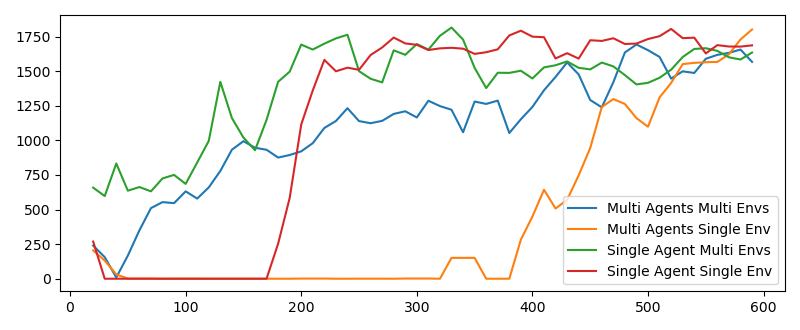
\includegraphics[width=\linewidth]{figures/5_evaluation_figs/env_agent_num_training_fig/num_completed_tasks.png}
    \caption{Environment and number of Agents - Number of completed tasks (Multi-env settings)}
    \label{fig:multi-env-num-completed-tasks}
\end{figure}

\begin{figure}[H]
    \centering
    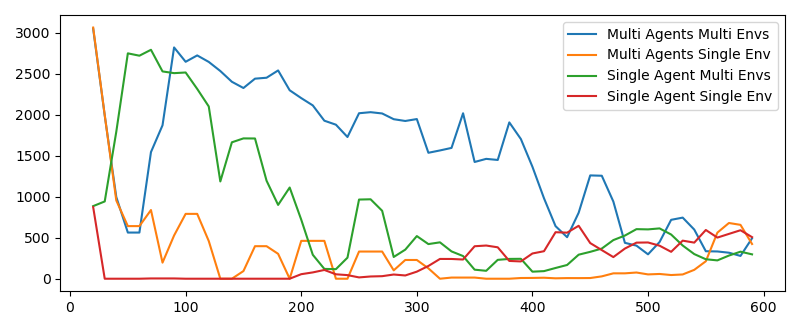
\includegraphics[width=\linewidth]{figures/5_evaluation_figs/env_agent_num_training_fig/num_failed_tasks.png}
    \caption{Environment and number of Agents - Number of failed tasks (Multi-env settings)}
    \label{fig:multi-env-num-failed-tasks}
\end{figure}

\begin{figure}[H]
    \centering
    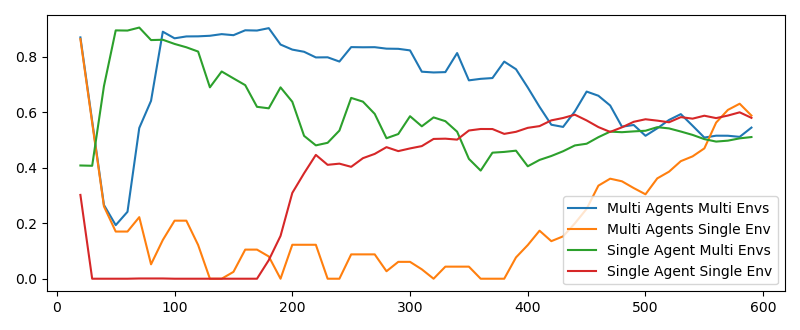
\includegraphics[width=\linewidth]{figures/5_evaluation_figs/env_agent_num_training_fig/percent_tasks.png}
    \caption{Environment and number of Agents - Percentage of tasks attempted (Multi-env settings)}
    \label{fig:multi-env-percent-tasks}
\end{figure}

In Figure~\ref{fig:multi-env-num-completed-tasks}, agents trained using only a single environment settings, both
single and multiple agents variations, took a relatively long time (150 and 350 episodes) for the agents to achieve 25\%
of its final total tasks completed. In comparison, both multi-environment agents achieved similar results within 50
episodes.

Despite the training speed of the single environment agents, after 600 episodes of training time, all agents no matter
the training environments or number of agents trained together achieve very similar results in all metrics
(figure~\ref{fig:multi-env-num-completed-tasks},~\ref{fig:multi-env-num-failed-tasks} and~\ref{fig:multi-env-percent-tasks}.
This is surprising that despite single environment agents not being trained on the multi-environment settings, they
achieve similar results as multi-environment agents. This means agents are able to generalised to unknown environment
effectively alas not as quickly. However more training is required to check if overfitting affects the performance as
the agent over learns a particular setting.

This also shows that single agent trained to the same level as multiple agents training together achieve similar
results. Meaning that showing that single agent can learn the optimal strategy without needing a  diverse "genetic"
pool of the multiple agents to train quickly.

\begin{figure}[H]
    \centering
    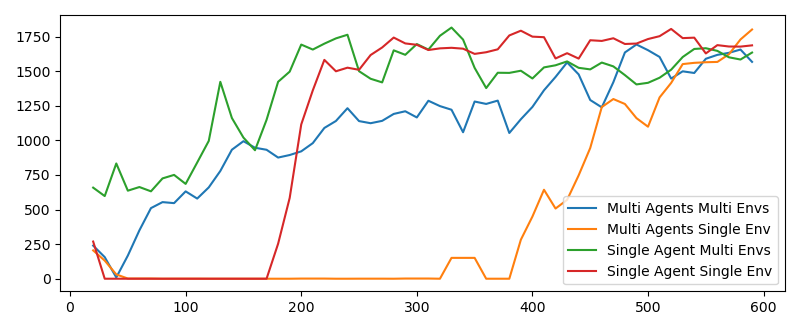
\includegraphics[width=\linewidth]{figures/5_evaluation_figs/env_agent_num_training_fig/single_env_num_completed_tasks.png}
    \caption{Environment and number of Agents - Number of completed tasks (Single env settings)}
    \label{fig:single-env-num-completed-tasks}
\end{figure}

\begin{figure}[H]
    \centering
    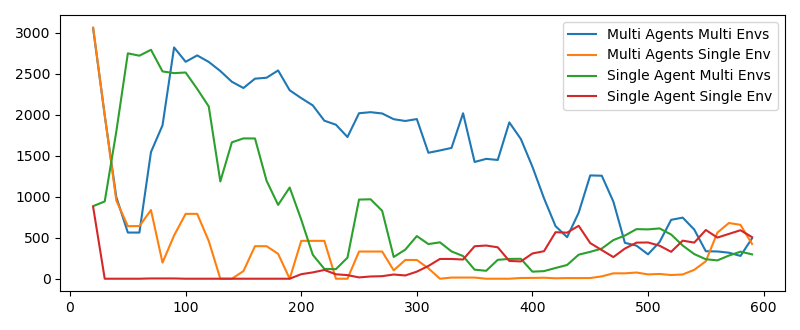
\includegraphics[width=\linewidth]{figures/5_evaluation_figs/env_agent_num_training_fig/single_env_num_failed_tasks.png}
    \caption{Environment and number of Agents - Number of failed tasks (Single env settings)}
    \label{fig:single-env-num-failed-tasks}
\end{figure}

\begin{figure}[H]
    \centering
    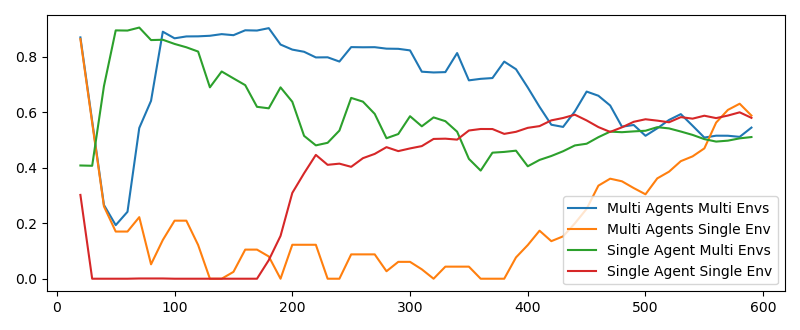
\includegraphics[width=\linewidth]{figures/5_evaluation_figs/env_agent_num_training_fig/single_env_percent_tasks.png}
    \caption{Environment and number of Agents - Percentage of tasks attempted (Single env settings)}
    \label{fig:single-env-percent-tasks}
\end{figure}

During training, all agents were simultaneously evaluated on the single environment setting as well as the
multi-environment settings, shown in Figures~\ref{fig:single-env-num-completed-tasks},
~\ref{fig:single-env-num-failed-tasks} and~\ref{fig:single-env-percent-tasks}. For the single environment agents, they
achieve 10\% more completed tasks than the multiple environment agents. This is understandable due to single environment
being more "specialised" for the single environment than multi-environment agents. As a result, this allows the single
environment agents to maximise profits in specialised environments compared to the multi-environment agents that have
learnt to maximise profit over more environments being less "specialised" for a single environment.

\subsection{Training Reinforcement Learning Algorithms}
\label{subsec:training-reinforcement-learning-algorithms}
To compare Reinforcement Learning algorithms, set out in Table~\ref{tab:reinforcement-learning-algorithms},
each were trained using the algorithms for both auctioning and resource allocation. During training, multiple
environments were used for both training and evaluation with three task pricing agents and a single resource allocation
agents. This was done because of the analyse in in Subsection~\ref{subsec:environment-and-agent-number-training}.

\begin{figure}[H]
    \centering
    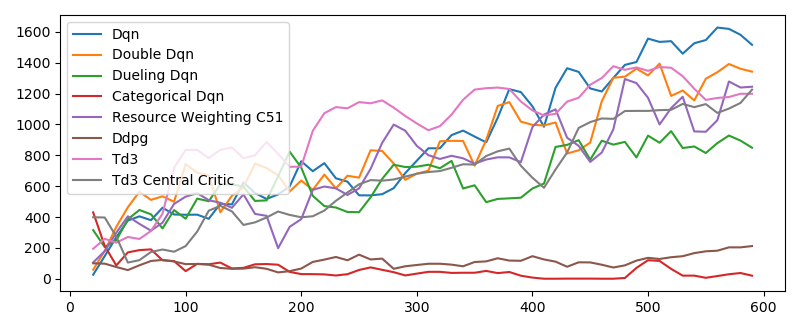
\includegraphics[width=\linewidth]{figures/5_evaluation_figs/algo_training_fig/num_completed_tasks.png}
    \caption{Reinforcement Learning algorithms - Number of completed tasks}
    \label{fig:algo-num-completed_tasks}
\end{figure}

\begin{figure}[H]
    \centering
    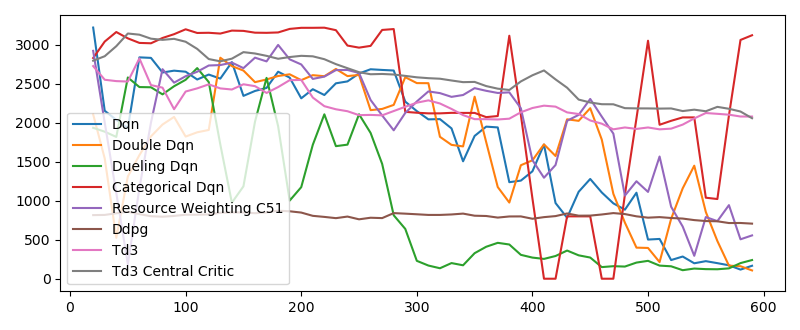
\includegraphics[width=\linewidth]{figures/5_evaluation_figs/algo_training_fig/num_failed_tasks.png}
    \caption{Reinforcement Learning algorithms - Number of failed tasks}
    \label{fig:algo-num-failed-tasks}
\end{figure}

\begin{figure}[H]
    \centering
    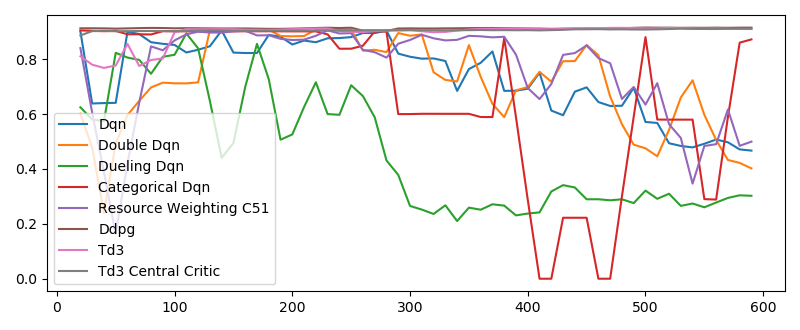
\includegraphics[width=\linewidth]{figures/5_evaluation_figs/algo_training_fig/percent_tasks.png}
    \caption{Reinforcement Learning algorithms - Percentage of tasks attempted}
    \label{fig:algo-percent-tasks}
\end{figure}

For the Dqn agents, the results did not match expectation as the heuristic Dqn agents achieved fewer completed tasks,
Figure~\ref{fig:algo-num-completed_tasks}, compared to the standard Dqn agent. This is surprising as previous
research~\citep{doubledqn, duelingdqn, rainbow} have found they to achieve better results than the standard Dqn,
despite no changes being made to the agents hyperparameters. Possible reasons for this is due to an incorrect
implementation, training time or initial network weights. While it is possible to be an incorrect implementation, this
is unlikely due to the code matching other implementation. The initial network weights could be a problem,
as when the best action is not the optimal actions can cause the network to be trained incorrect at the start but this
will self-correct given enough time. Therefore training time is believed to be the primary reason for the heuristic Dqn
agents achieving worse result. For future works, doubling the number of training episodes is proposed because of this.

The Categorical Dqn agent struggled to achieving over 50 completed tasks during evaluation after 600 episodes of
training. However the reason for this is unknown as a separate training was done using a Dqn for the task pricing and
a Categorical Dqn agent for the resource allocation, referred to as 'Resource Weighting C51'. This agent was able to
achieve similar results to the other Dqn agent meaning that the task pricing agent fails to work with the Categorical
Dqn agent. The reason for this is believed to be due to agent min and max value hyperparameters not due to the
implementation. But further research is required to explore Categorical Dqn agents fully and understand
why for task pricing this has not worked.

Figure~\ref{fig:algo-percent-tasks} shows that the Ddpg agents (Ddpg, Td3, Td3 Central critic) attempted over 80\% of
auctioned tasks compared to the Dqn agents with only 60\%. As a result, agent's can't distributed resource to
each of its tasks meaning that the agents have a significantly higher number of failed tasks
(Figure~\ref{fig:algo-num-failed-tasks}) in comparison to Dqn agent. In terms of completed tasks, the Td3 and Td3
central critic (where all task pricing agents use the same critic and twin critic) are able to achieve results as good
as the Dqn agent. This is in comparison to the Ddpg agent which struggled to complete 25\% of the amount achieved by
the other agents showing that the twin critic heuristics are highly effective for the Ddpg agents.

%\begin{figure}[H]
%    \centering
%    \begin{minipage}{0.5\textwidth}
%        \centering
%        \includegraphics[width=1.0\textwidth]{figures/5_evaluation_figs/algo_training_fig/dqn_auction_prices.png}
%        \caption{Deep Q Network auction prices}
%        \label{fig:dqn-auction-prices}
%    \end{minipage}\hfill
%    \begin{minipage}{0.5\textwidth}
%        \centering
%        \includegraphics[width=1.0\textwidth]{figures/5_evaluation_figs/algo_training_fig/dqn_weightings.png}
%        \caption{Deep Q Network resource weightings}
%        \label{fig:dqn-resource-weightings}
%    \end{minipage}
%\end{figure}

\subsection{Training Neural Network Architectures}
\label{subsec:neural-network-architecture-training}
There are a wide-range of compatible neural network architectures that agents can use, as outlined in
Table~\ref{tab:neural-network-layers}. To compare these architectures, five different network architectures are trained:
RNN, LSTM, GRU, Bidirectional using an LSTM network and
a Seq2Seq network. These networks are trained using the Dqn algorithm due to its constant performance compared to the
Ddpg agents as shown in the previous section. The Seq2Seq network used a Dqn Agent with a LSTM network for the task
pricing agent and the Seq2Seq network with a Td3 agent for resource allocation. This is as the network architecture is
only applicable for the resource weighting agent and requires a policy gradient algorithm to train.

\begin{figure}[H]
    \centering
    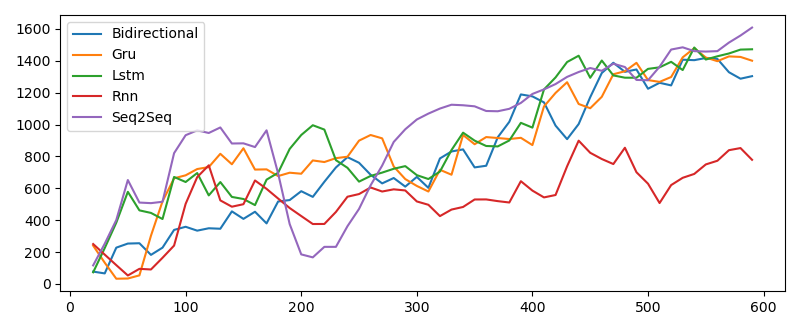
\includegraphics[width=\linewidth]{figures/5_evaluation_figs/net_arch_training_fig/num_completed_tasks.png}
    \caption{Network Architecture - Number of completed tasks}
    \label{fig:net_arch_num_completed_tasks}
\end{figure}

\begin{figure}[H]
    \centering
    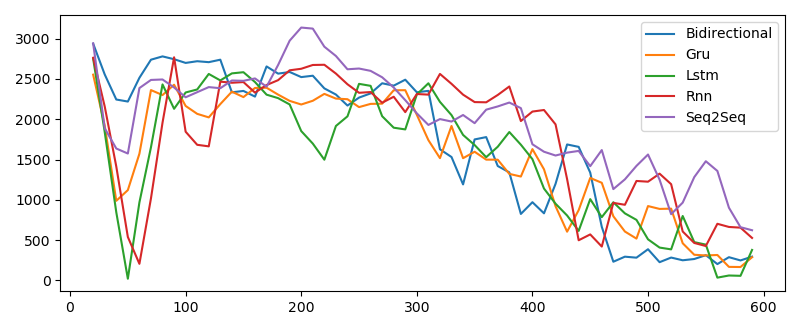
\includegraphics[width=\linewidth]{figures/5_evaluation_figs/net_arch_training_fig/num_failed_tasks.png}
    \caption{Network Architecture - Number of failed tasks}
    \label{fig:net_arch_num_failed_tasks}
\end{figure}

\begin{figure}[H]
    \centering
    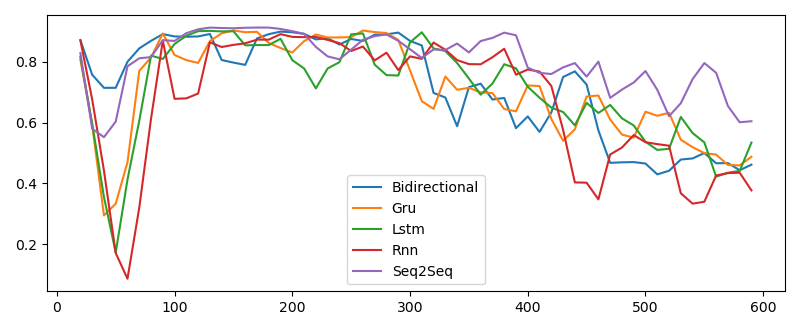
\includegraphics[width=\linewidth]{figures/5_evaluation_figs/net_arch_training_fig/percent_tasks.png}
    \caption{Network Architecture - Percent of tasks attempted}
    \label{fig:net_arch_percent_tasks}
\end{figure}

Figure~\ref{fig:net_arch_num_completed_tasks} shows that the LSTM, GRU, Bidirectional and Seq2Seq networks all
achieved a similar score in the number of tasks completed while the RNN network achieves 30\% less. RNNs have a known
problem of vanishing or exploding gradients as explained in Table~\ref{tab:neural-network-layers} making it
understandable why the network struggled. \\
These results are slightly surprising that the heuristic advantages of LSTM and Bidirectional over GRU are not required
for agents to approximate the optimal strategy. While ability for the Seq2Seq to learn the task policies together is not
a large advantage for the agents in comparison to the other network that weighted tasks individually. However
more training time is required till all agents plateau in training which could allow the more complex networks to
accel.
